% Lecture for ph2a Caltech 2017: Vibrations and Waves
\documentclass[pdf,hideothersubsections]{beamer}
\usepackage{beamerthemeshadow}
\mode<presentation>
  {
    \usefonttheme{structuresmallcapsserif}
    \usetheme{PaloAlto}
    \usecolortheme{seagull}
    %\useinnertheme{circles}
%    \useoutertheme{tree}
  }

\usepackage{svg}
\usepackage{xmpmulti}

\usepackage{hyperref}
\hypersetup{
    pdffitwindow=true,     % window fit to page when opened
    colorlinks=true,       % false: boxed links; true: colored links
    linkcolor=orange,          % color of internal links (change box color with linkbordercolor)
    citecolor=green,        % color of links to bibliography
    filecolor=magenta,      % color of file links
    urlcolor=blue           % color of external links
}

% Fonts/encoding
\renewcommand{\UrlFont}{\tiny}
\usepackage[utf8]{inputenc}
\usepackage[T1]{fontenc}
%\usepackage[sc,medium,raggedright]{titlesec}
\usepackage{newtxmath}
%\usepackage{libertine}
\usepackage[osf]{ebgaramond}

\graphicspath{{Figures/}}

\begin{document}
\title{Driven Oscillations and Resonance}  
\author{Caltech: ph2a}
\date{5 - Oct - 2017}
%\logo{
\includegraphics[height=0.5cm]{../caltech_logo.png}}

\frame{\titlepage} 

\frame{\frametitle{Table of contents}\tableofcontents} 

\setbeamerfont{footnote}{size=\tiny}

\section{Previous Summary}
\begin{frame}
\frametitle{Recently}
\begin{itemize}
\item Q is a measure of the 'Quality' of an oscillator; how long it
  takes to ring down: $Q = \omega_0 \tau / 2$
\pause
\item Air track demo shows how this effect works for a driven oscillator
\pause
\end{itemize}
\end{frame}


\section{Damped Oscillations}
\begin{frame}
\frametitle{Review: Complex sol. for damped SHO}
Use the same approach as before:
\begin{itemize}
\item $L \ddot{Q} + R \dot{Q} + Q/C = 0$
\pause
\item $\tilde{Q}(t) = A e^{i (\omega t + \phi_0)}$
\pause
\item $-L \omega^2 \tilde{Q} + i \omega R \tilde{Q} + \tilde{Q}/C = 0$
\end{itemize}
\pause
Dividing by $L \tilde{Q}$, we get a quadratic equation for $\omega$: \\
\pause
\begin{center}
$\omega = \sqrt{\omega_0^2 - \Big(\frac{R}{2 L}\Big)^2} + i \frac{R}{2 L}$ \\
\end{center}
\pause
Let's call the real part $\omega$ and plug back into the guess for Q(t):
\pause
\begin{center}
$\tilde{Q} = A e^{i (\omega t + \phi_0)} e^{-(R/2 L) t}$\\
\end{center}
\pause
We can define the time constant: $\tau \equiv 2 L/R$, so that: \\
\pause
Taking the real part, we find the solution as before (with the damping): \\
\pause
\begin{center}
$Re\left\{\tilde{Q}\right\} = Q = A \cos(\omega t + \phi_o) e^{-t/\tau}$
\end{center}

\end{frame}

\subsection{Classes of Damping}
\begin{frame}
\frametitle{Under, Over, \& Critical Damping}
\pause
The complex angular frequency of the oscillator:

\begin{center}
$\omega = \sqrt{\omega_0^2 - \Big(\frac{R}{2 L}\Big)^2} + i \frac{R}{2 L}$ \\
\end{center}
\pause
\begin{block}{Definitions}
Under: $\Big(\frac{R}{2 L}\Big)^2 < \omega_0^2  \implies
Re\left\{\omega\right\} > 0$ \\
Critical: $\Big(\frac{R}{2 L}\Big)^2 = \omega_0^2 \implies
Re\left\{\omega\right\} = 0$ \\
Over: $\Big(\frac{R}{2 L}\Big)^2 > \omega_0^2 \implies
Re\left\{\omega\right\} = 0$
\end{block}


\end{frame}


\subsection{Quality Factor}
\begin{frame}
\frametitle{The Quality Factor: I}
\pause
\begin{block}{Definition I:}
$Q \equiv 2 \pi \frac{\rm energy~stored}{\rm energy~dissipated~per~cycle}$
\end{block}
\pause
\begin{block}{Definition II:}
$Q \simeq \omega_0 \tau / 2$ \\
-- accurate for high Q\footnotemark systems
\end{block}

\footnotetext[1]{Not to be confused with 'Q' as a variable indicating charge! }

\end{frame}

\begin{frame}
\frametitle{Decaying Oscillation}

\centering
\includegraphics[width=0.75\textwidth]{damped_sine_wave.pdf}

\end{frame}



\begin{frame}
\frametitle{The Quality Factor: II}

\begin{block}{Definition II:}
$Q \equiv \frac{\omega_R}{\Delta \omega}$
\end{block}
\pause
\centering
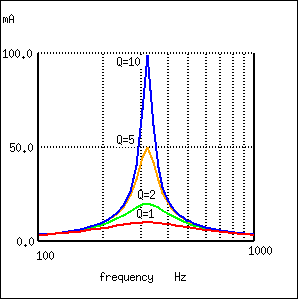
\includegraphics[width=0.35\textwidth]{LorentzianQ.png}

Demo: Air Track with magnets and \emph{lasers}.

\end{frame}



\begin{frame}
\frametitle{The Quality Factor: Examples}

The Q of some common household items:
\begin{table}
\centering
    \resizebox{\columnwidth}{!}{%
    \begin{tabular}{|l|c|r|}
      \hline
    Item Name                     & Frequency (Hz)  & Quality Factor \\ \hline
    Rubber Stopper                       & 10       & 0.5      \\
    Church Bell (Cologne)                & 330      & 1500     \\
    Stop Sign (hit with a rubber mallet) & 200      & 1000     \\
    ${}_0S_0$ Dilational Mode of the Earth     & 0.0008   & 3000     \\
    75 mm silicon wafer                  & 800      & 50,000   \\
    Quartz Crystal Resonator             & 10$^6$   & $10^4$\,--\,$10^6$ \\
    Large, High Purity Glass             & 3000     & 10$^8$   \\ \hline
    \end{tabular}}
\end{table}



\end{frame}


\section{Energy of Oscillators}
\begin{frame}
\frametitle{Kinetic and Potential Energy}
\pause
\begin{enumerate}
\item Many systems in physics can be understood simply by
  understanding their energy relations.
\pause
\item For the SHO, the potential energy is simply: $U = \int{-F dx} =
  \frac{1}{2}k x^2$
\pause
\item As usual, the kinetic energy is just $\frac{1}{2} m v^2$
\pause
\item and so the total energy, $E =  \frac{1}{2} m v^2 + \frac{1}{2}k x^2$
\end{enumerate}

\end{frame}

\begin{frame}
\frametitle{Kinetic and Potential Energy}
Plugging in our guess for the SHO: $x = A cos(\omega t + \phi_0)$,
remembering that $\omega = \sqrt{k/m}$ and $sin^2 + cos^2 = 1$:
\begin{align*}
E  &= \frac{1}{2} \Big[ m v^2 + k x^2 \Big]             \\
   &= \frac{1}{2} A^2 \Big[m \omega^2 (sin(\omega t + \phi_0))^2 + k (cos(\omega t + \phi_0))^2 \Big]   \\
   &= \frac{1}{2} A^2 k \Big[(sin(\omega t + \phi_0))^2 + (cos(\omega t + \phi_0))^2 \Big]   \\
   &= \frac{1}{2} k A^2
\end{align*}
So the total energy of an \emph{undamped} SHO is a constant\footnotemark.

\footnotetext[1]{Emmy Noether's Theorem about conservation and
  symmetry is profound and wonderful. }

\end{frame}



%\section{The Drag Force as Damping}
%\begin{frame}
%\frametitle{A Model for Drag Force}
%\end{frame}




\section{Summary}
\begin{frame}
\frametitle{Summary}
\begin{enumerate}
\pause
\item For linear systems, the resultant of two vibrations is just their sum.
\pause
\item Sum of two oscillations with different frequencies leads to \emph{beats}.
\pause
\item In a conservative system, the energy relations determine the
  motions.
%\item Drag force
\end{enumerate}
\end{frame}


\end{document}

